\section*{圖片}

\begin{figure}[H]  % [H]固定figure於某一頁
\begin{center}
\caption{各變數時間趨勢} \label{trend}
	\begin{subfigure}[b]{0.65\textwidth}
	 	\caption{各商品銷售量時間趨勢} \label{trend_volume}
		\vspace{-0.85em}
	 	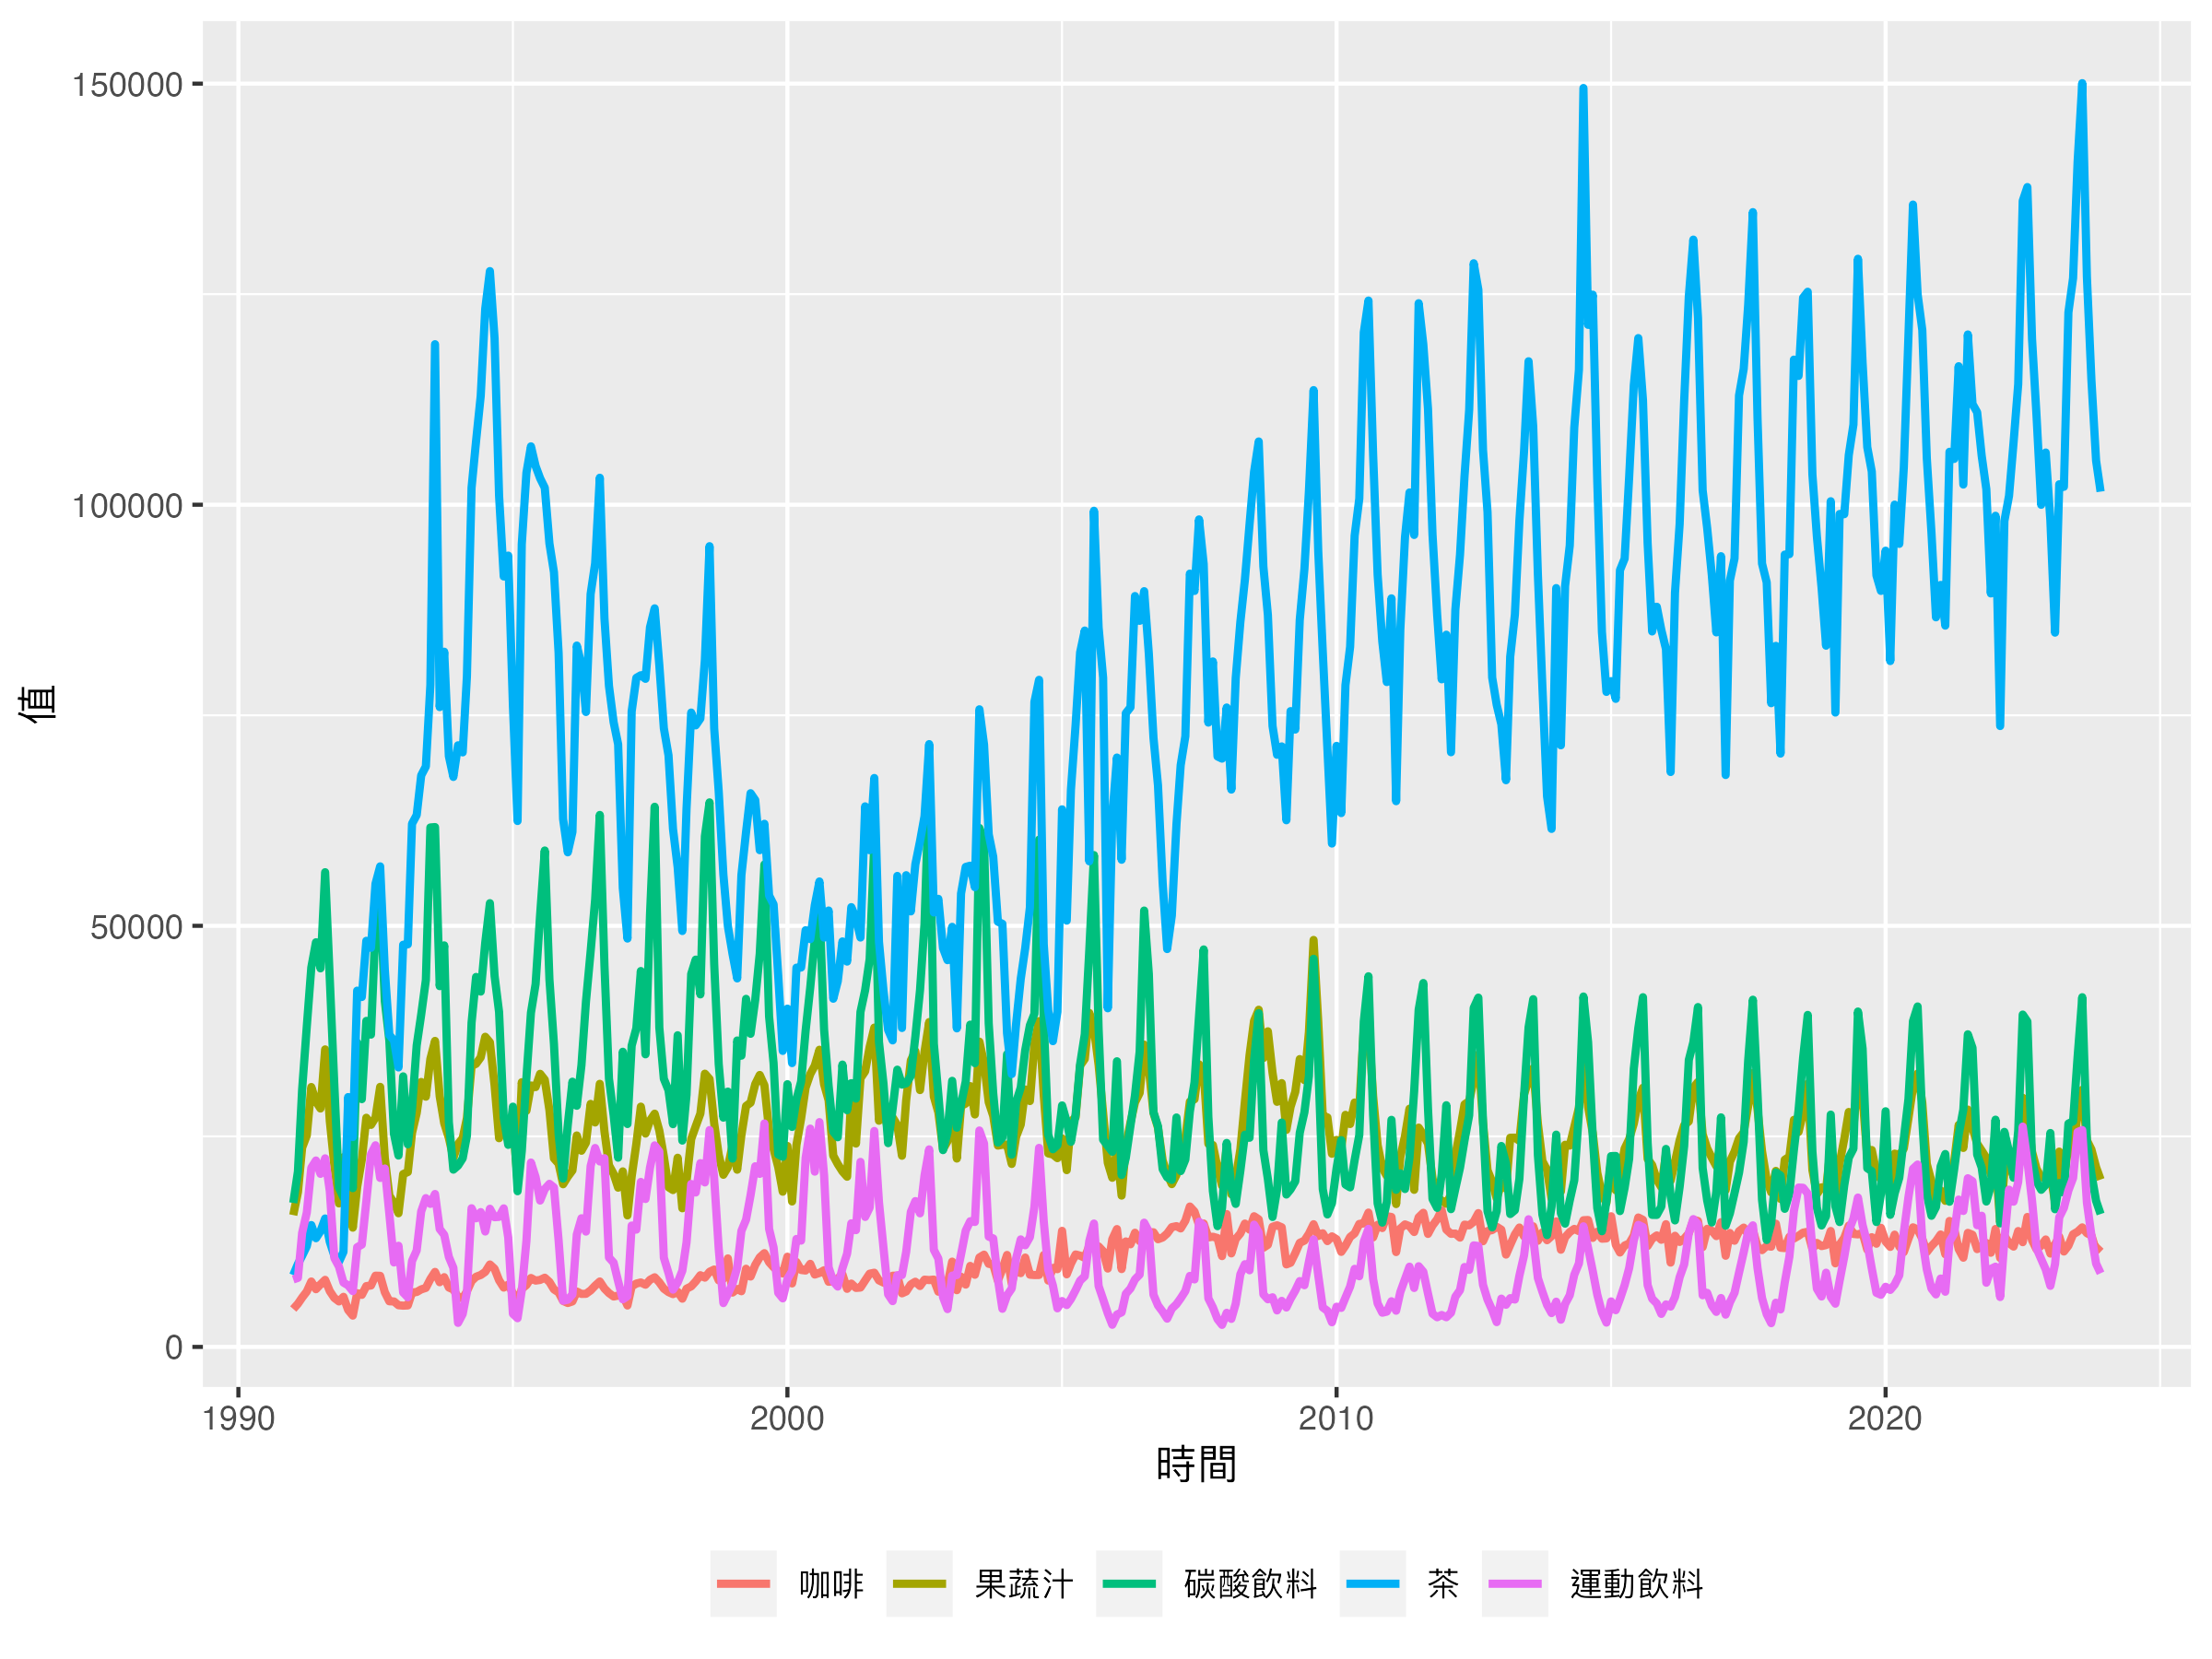
\includegraphics[width=\textwidth]{../outcome/chart1.png}  % both png, jpg can be used for graphs
	 \end{subfigure}
	 \begin{subfigure}[b]{0.65\textwidth}
		\caption{各商品價格時間趨勢} \label{trend_price}
		\vspace{-0.85em}
		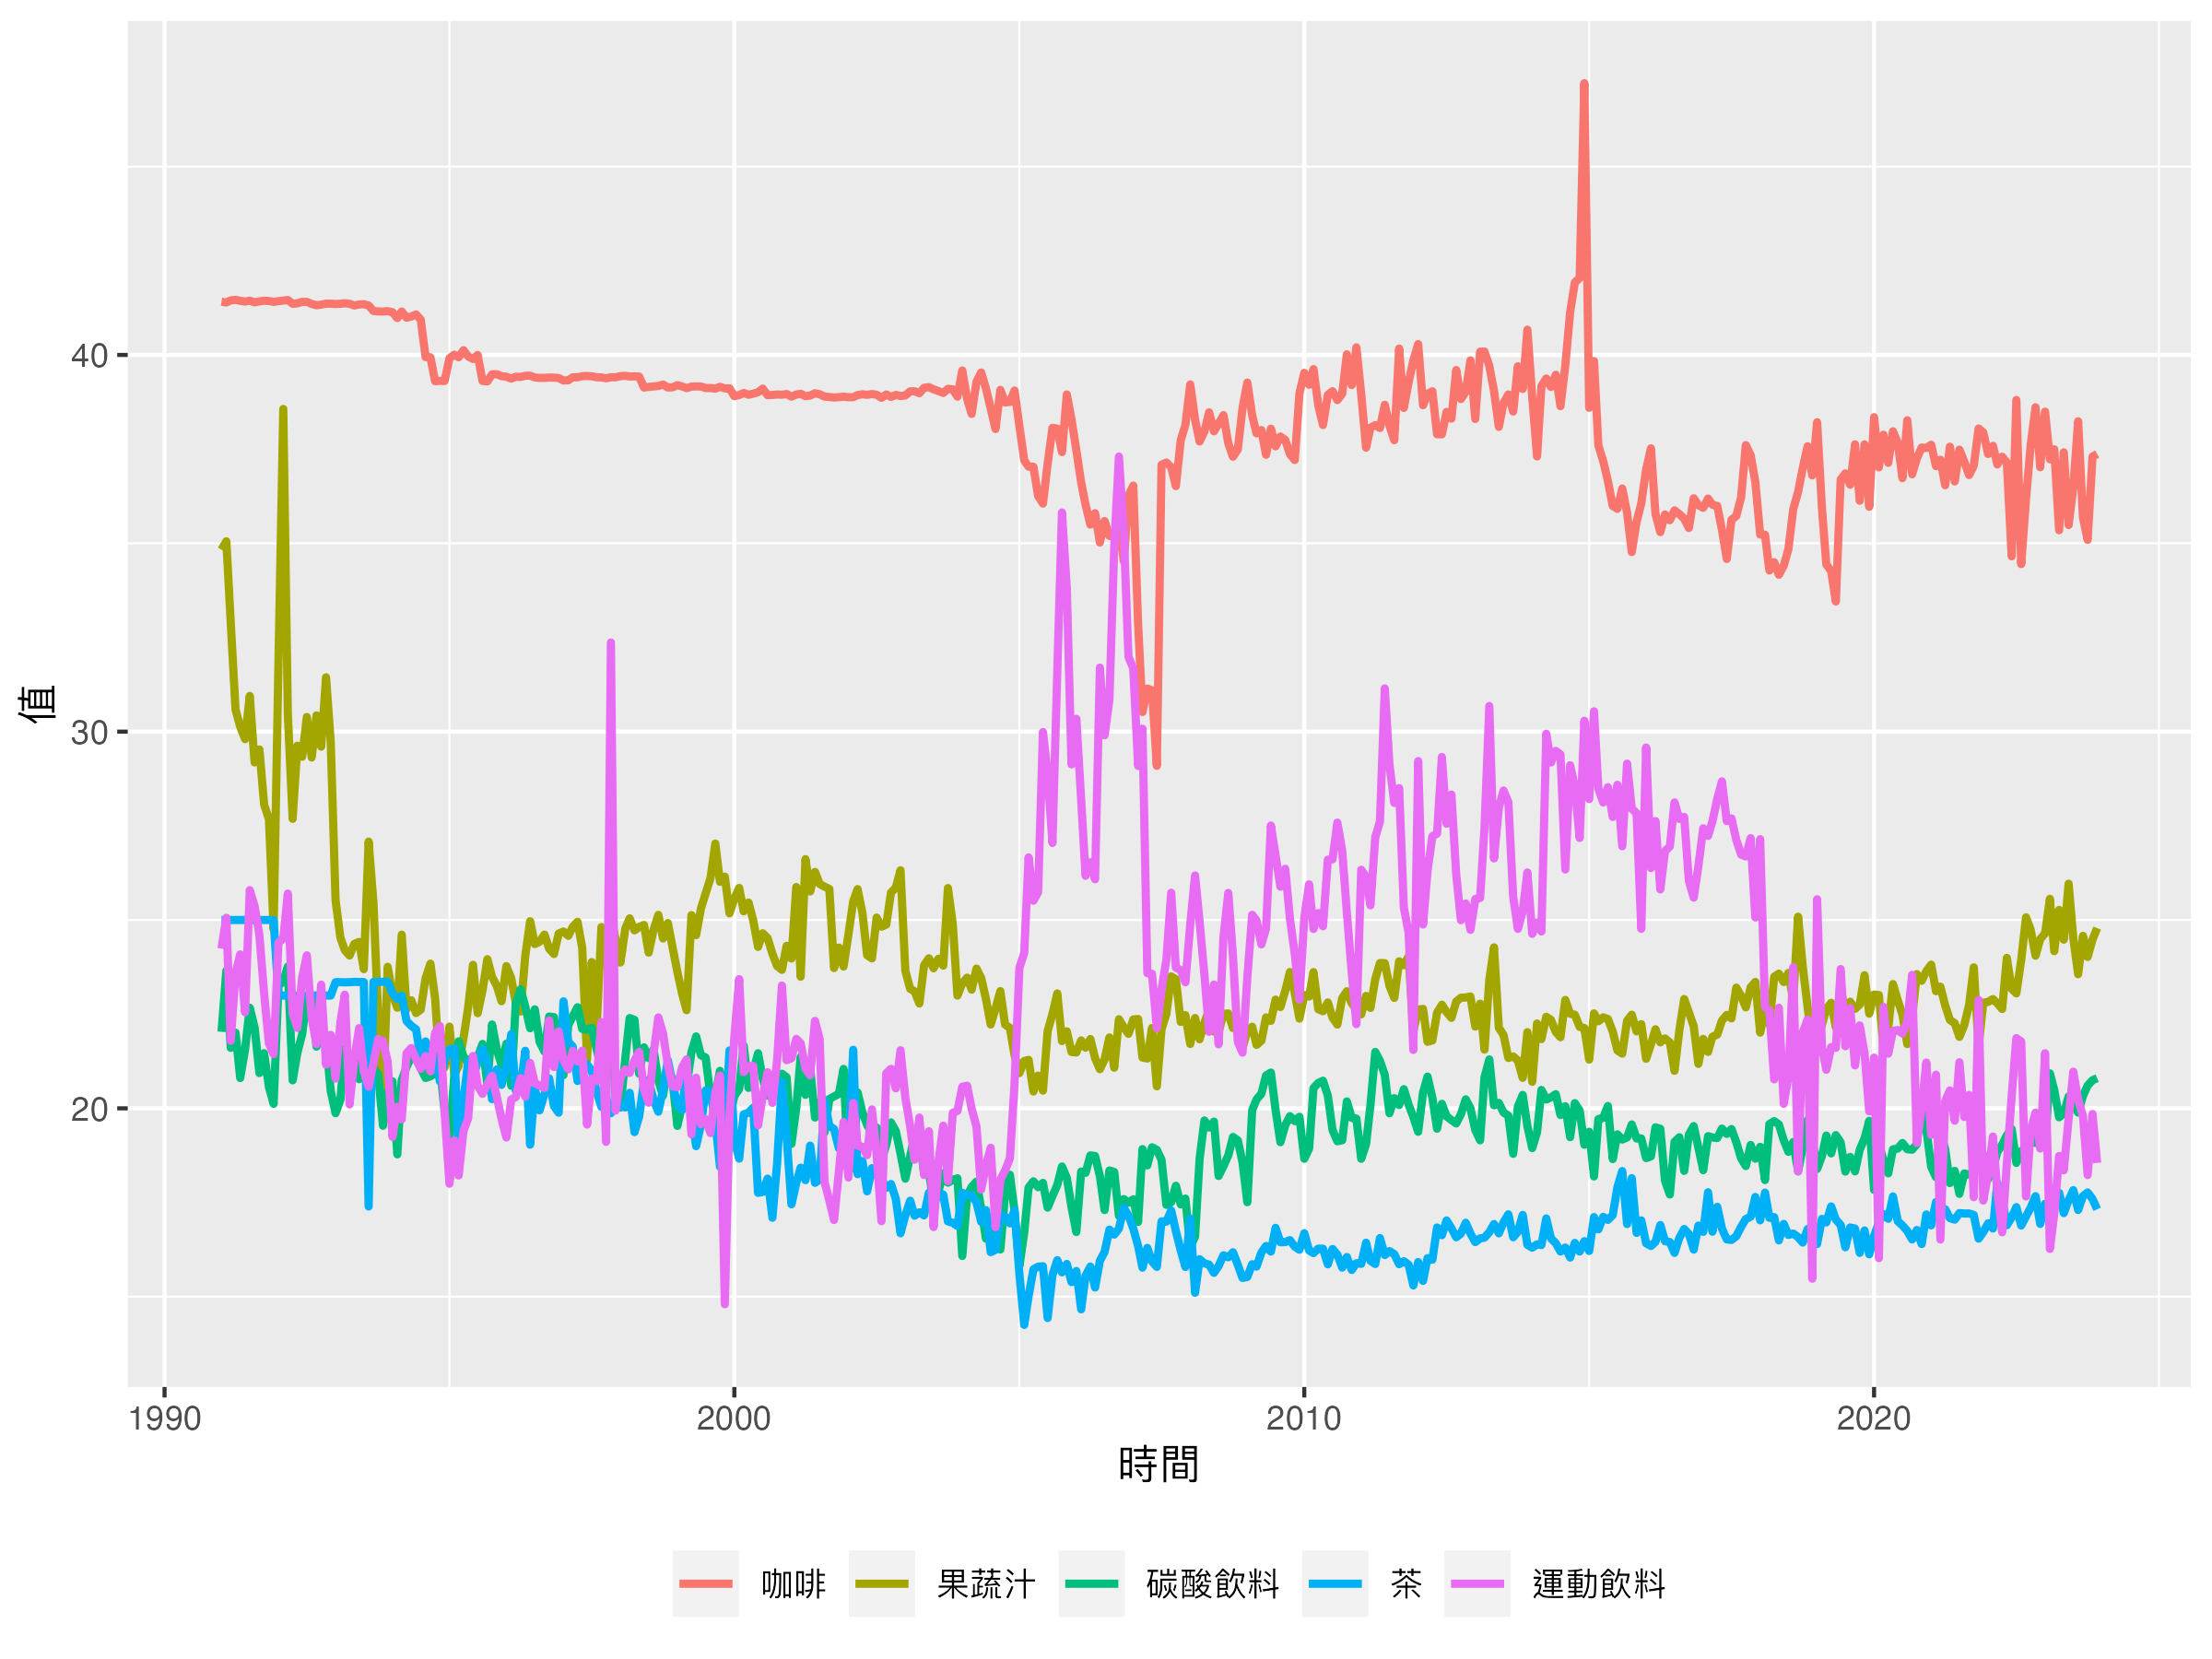
\includegraphics[width=\textwidth]{../outcome/chart2.png}
	\end{subfigure}
\end{center}
\end{figure}
\vspace{-3em}
\begin{singlespace}
        \begin{footnotesize}
        		\noindent {\it Notes:} \ref{trend}為各變數時間變動的趨勢,圖\ref{trend_volume}及圖\ref{trend_price}分別為各商品的銷售量與價格。在銷售量隨時間變化的的圖\ref{trend_volume}中,可以看到明顯的季節性波動,顯示各種飲料在每年都有其週期性,其中可以看到茶的銷售量位居所有飲料之冠。在價格方面,圖 \ref{trend_price}顯示以咖啡的單價最高。
        \end{footnotesize}
\end{singlespace}


\begin{figure}[H]  % [H]固定figure於某一頁
	\begin{center}
	\caption{各變數殘差自相關檢定 (ACF) 分析} \label{ACF}
		\begin{subfigure}[b]{0.65\textwidth}
			 \caption{AIDS模型} \label{ACF_aids}
			\vspace{-0.85em}
			 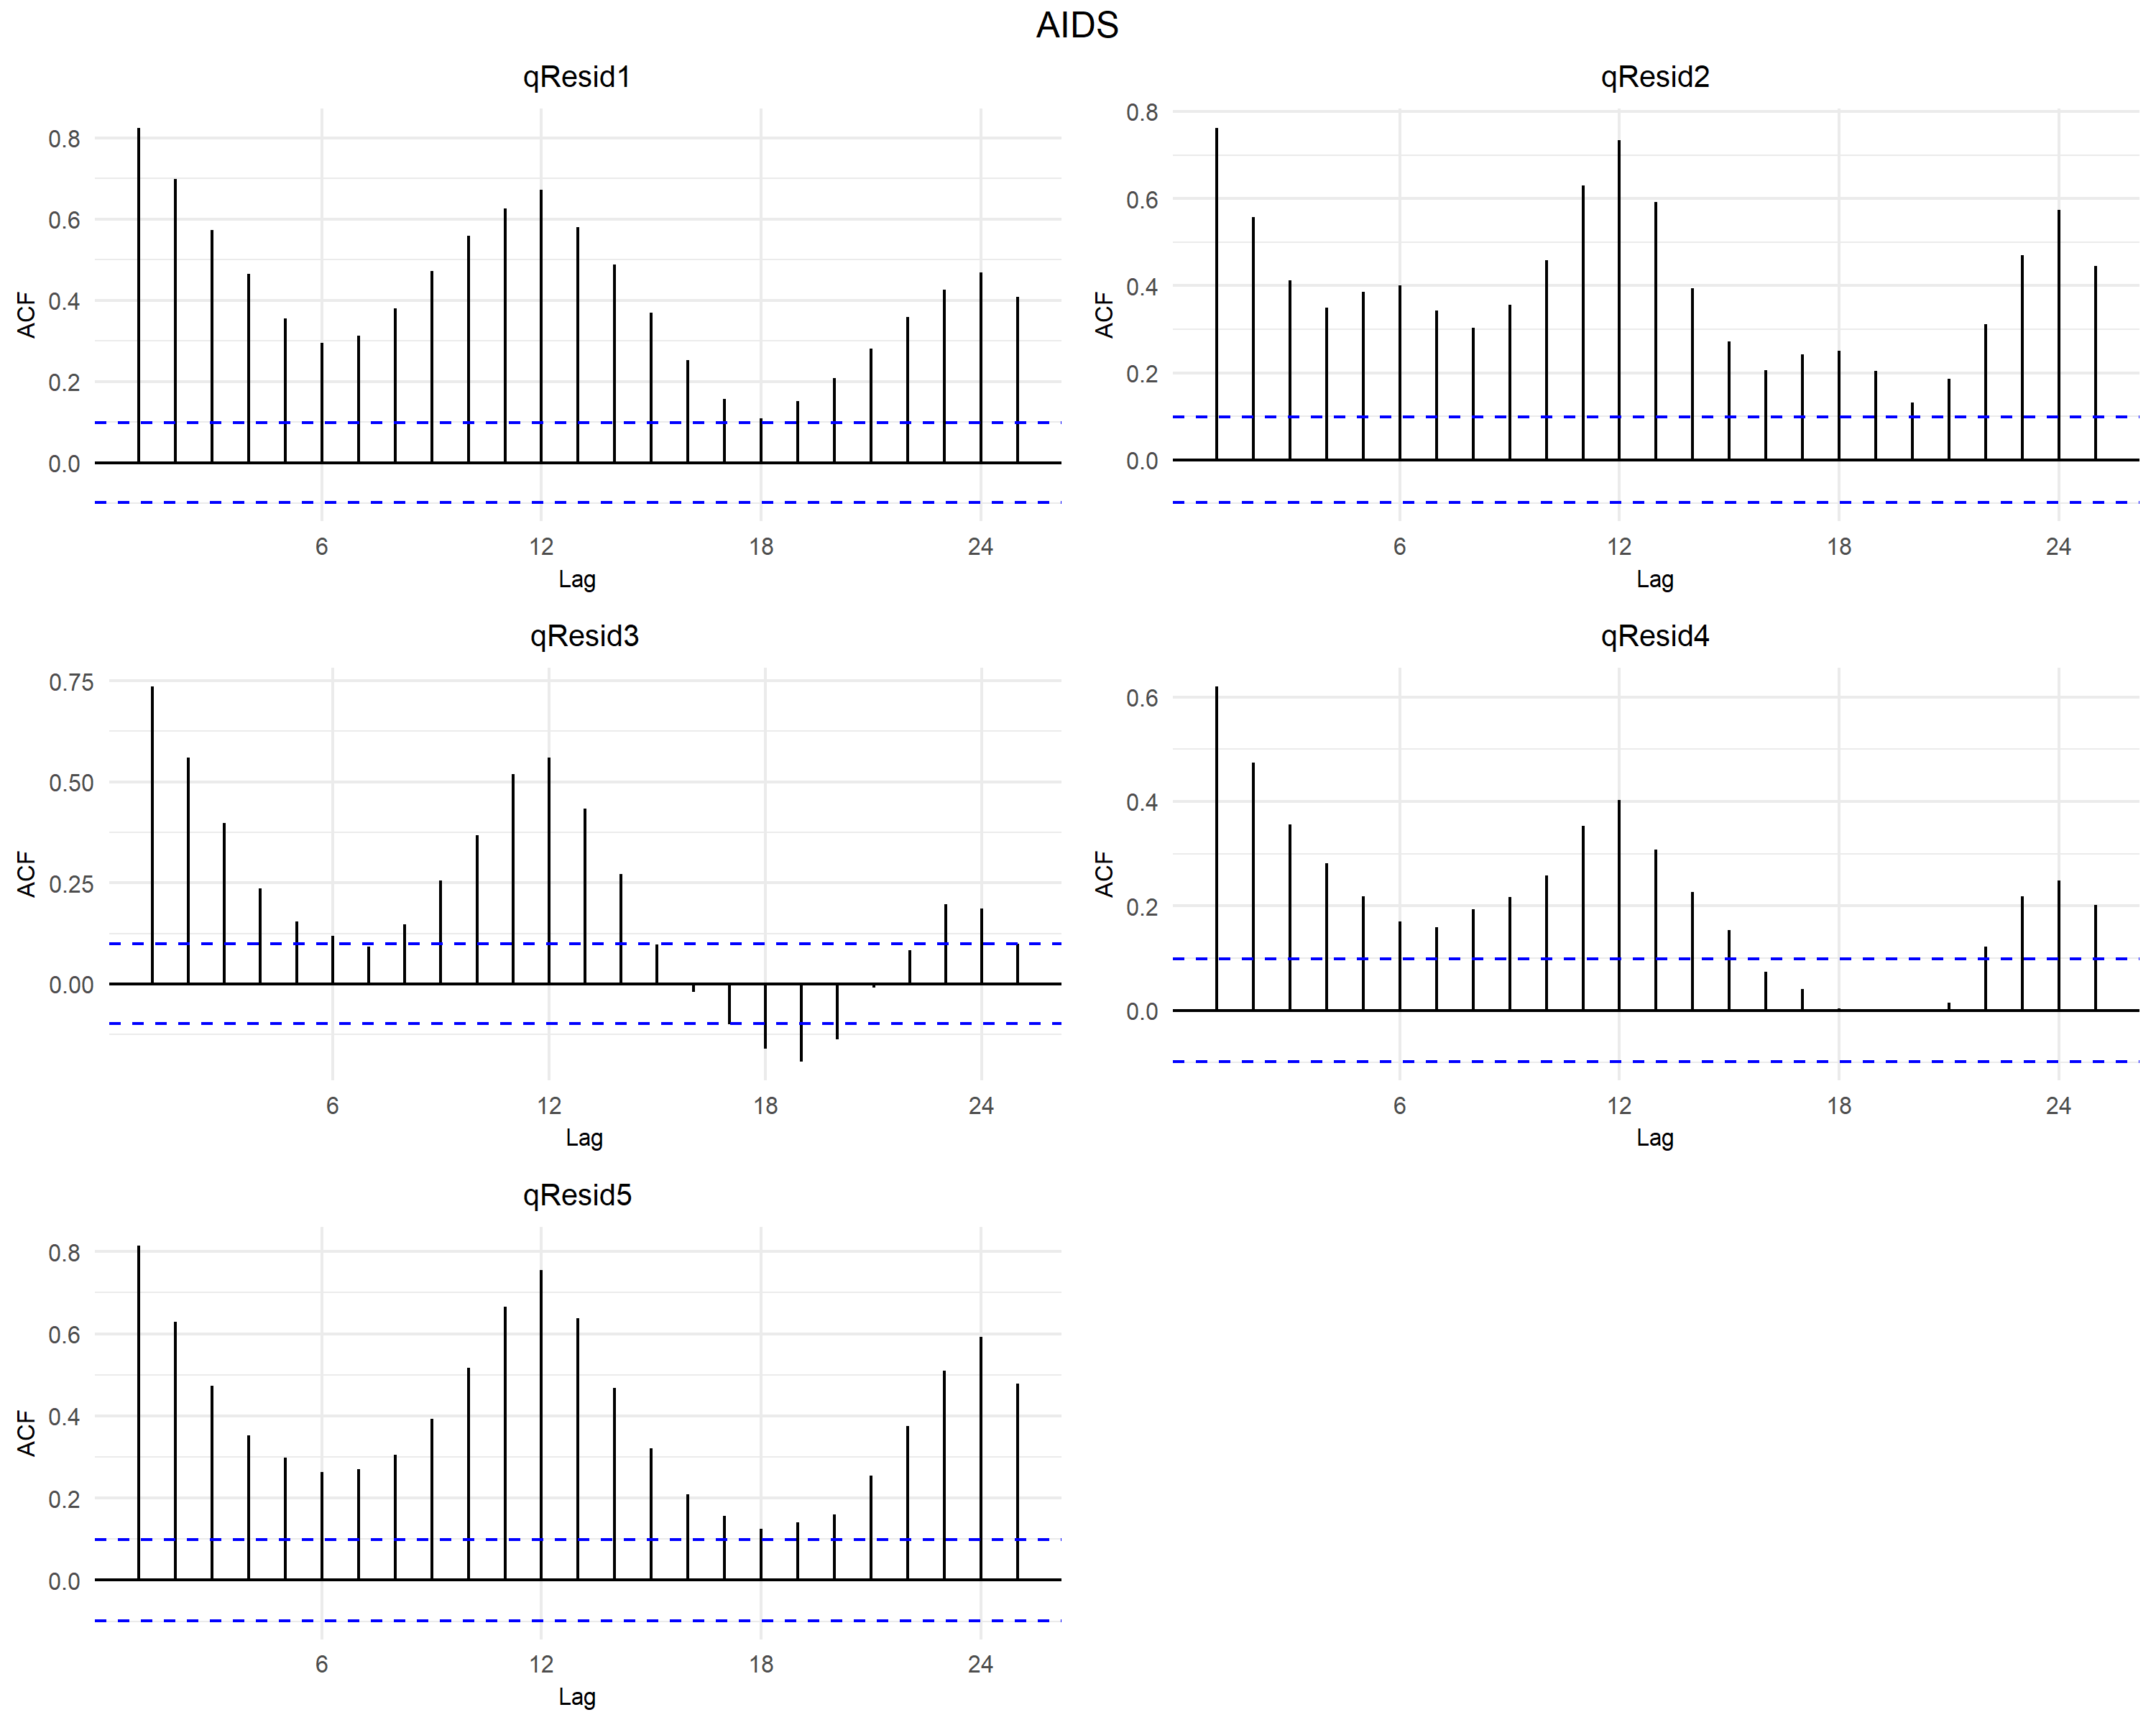
\includegraphics[width=\textwidth]{../outcome/AIDS_plot_qResid.png}  % both png, jpg can be used for graphs
		 \end{subfigure}
		 \begin{subfigure}[b]{0.65\textwidth}
			\caption{LAAIDS模型} \label{ACF_laaids}
			\vspace{-0.85em}
			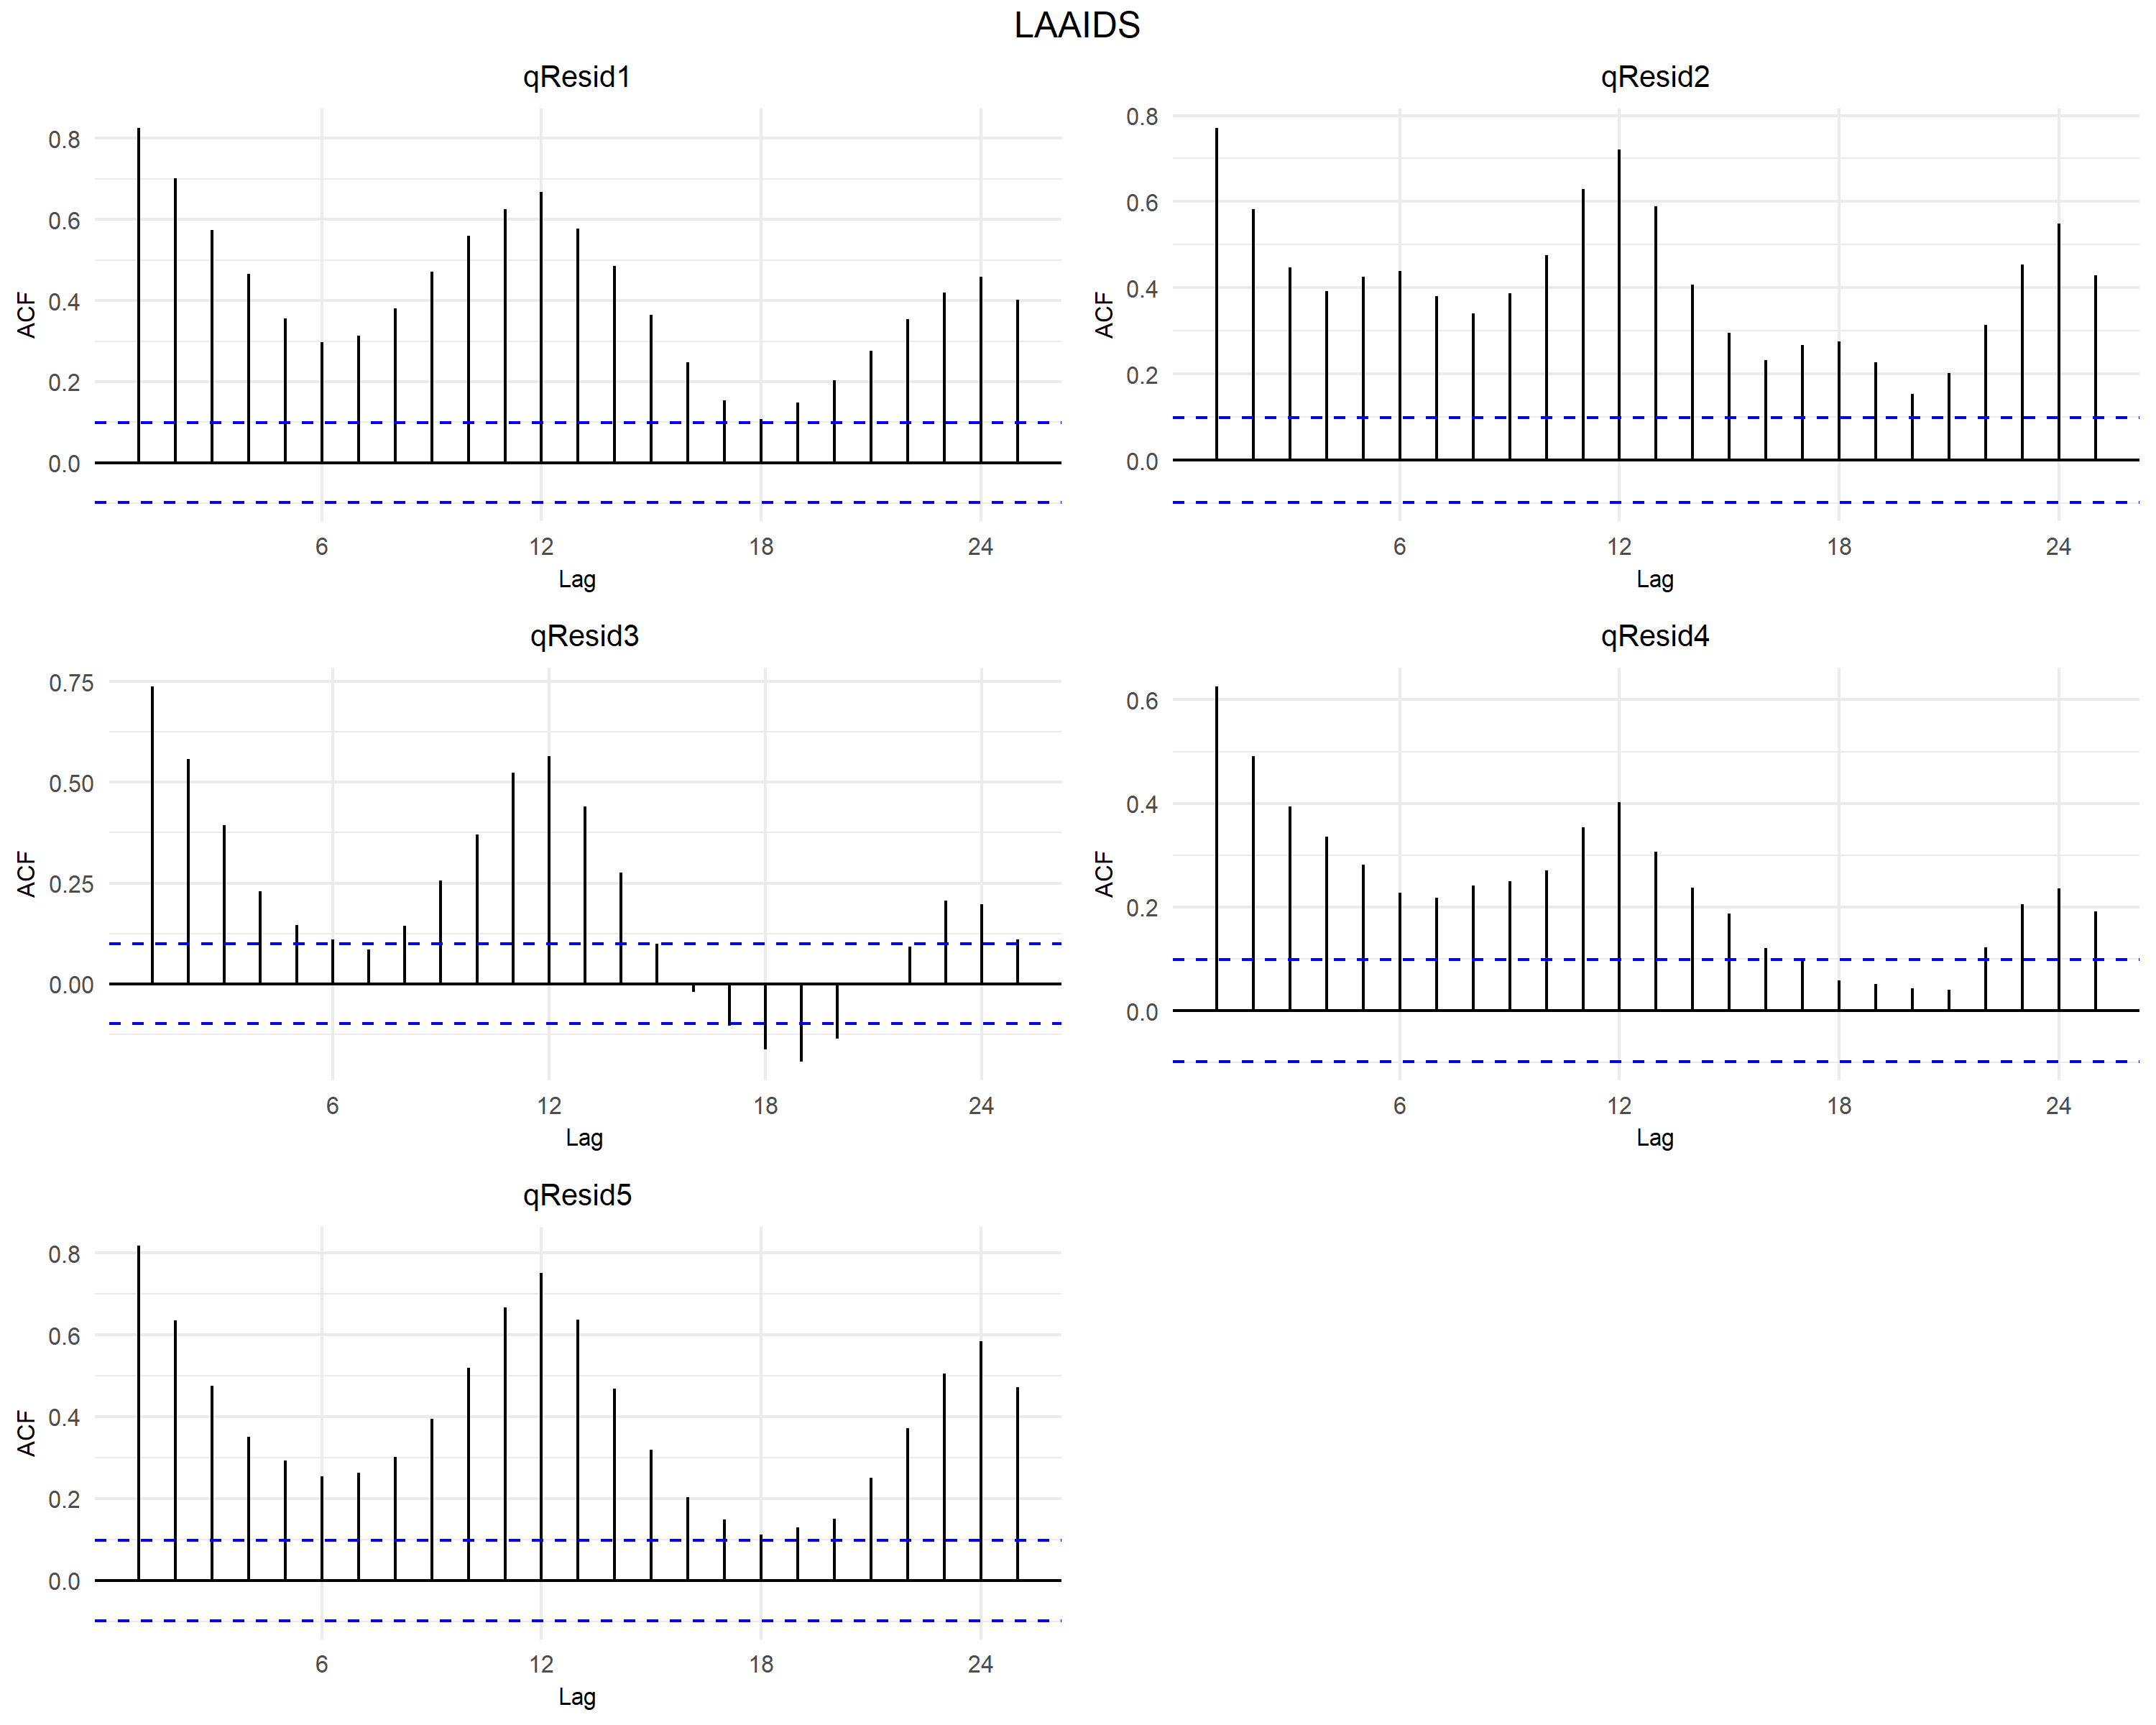
\includegraphics[width=\textwidth]{../outcome/LAAIDS_plot_qResid.png}
		\end{subfigure}
	\end{center}
\end{figure}
\vspace{-3em}
\begin{singlespace}
		\begin{footnotesize}
				\noindent {\it Notes:} qResid1 至 qResid5 分別為果蔬汁、碳酸飲料、運動飲料、咖啡飲料和茶飲料。
				在 AIDS 模型的 ACF 中,果蔬汁、碳酸飲料和茶飲料在低滯後期顯示顯著自相關,且自相關隨滯後增加呈周期性變化,可能與季節性消費相關。
				運動飲料和咖啡飲料在低滯後期的自相關顯著,但隨滯後增加逐漸衰減至不顯著。
				LAAIDS 模型的 ACF 與 AIDS 類似,但碳酸飲料和咖啡飲料的殘差自相關更強。
		\end{footnotesize}
\end{singlespace}



% \newpage
% \begin{figure}[H]
% 	\centering
% 	\caption{The Relationship Between GDP Per Capita and the Total Fertility Rate}\label{fig.gdp_fertility}
% 	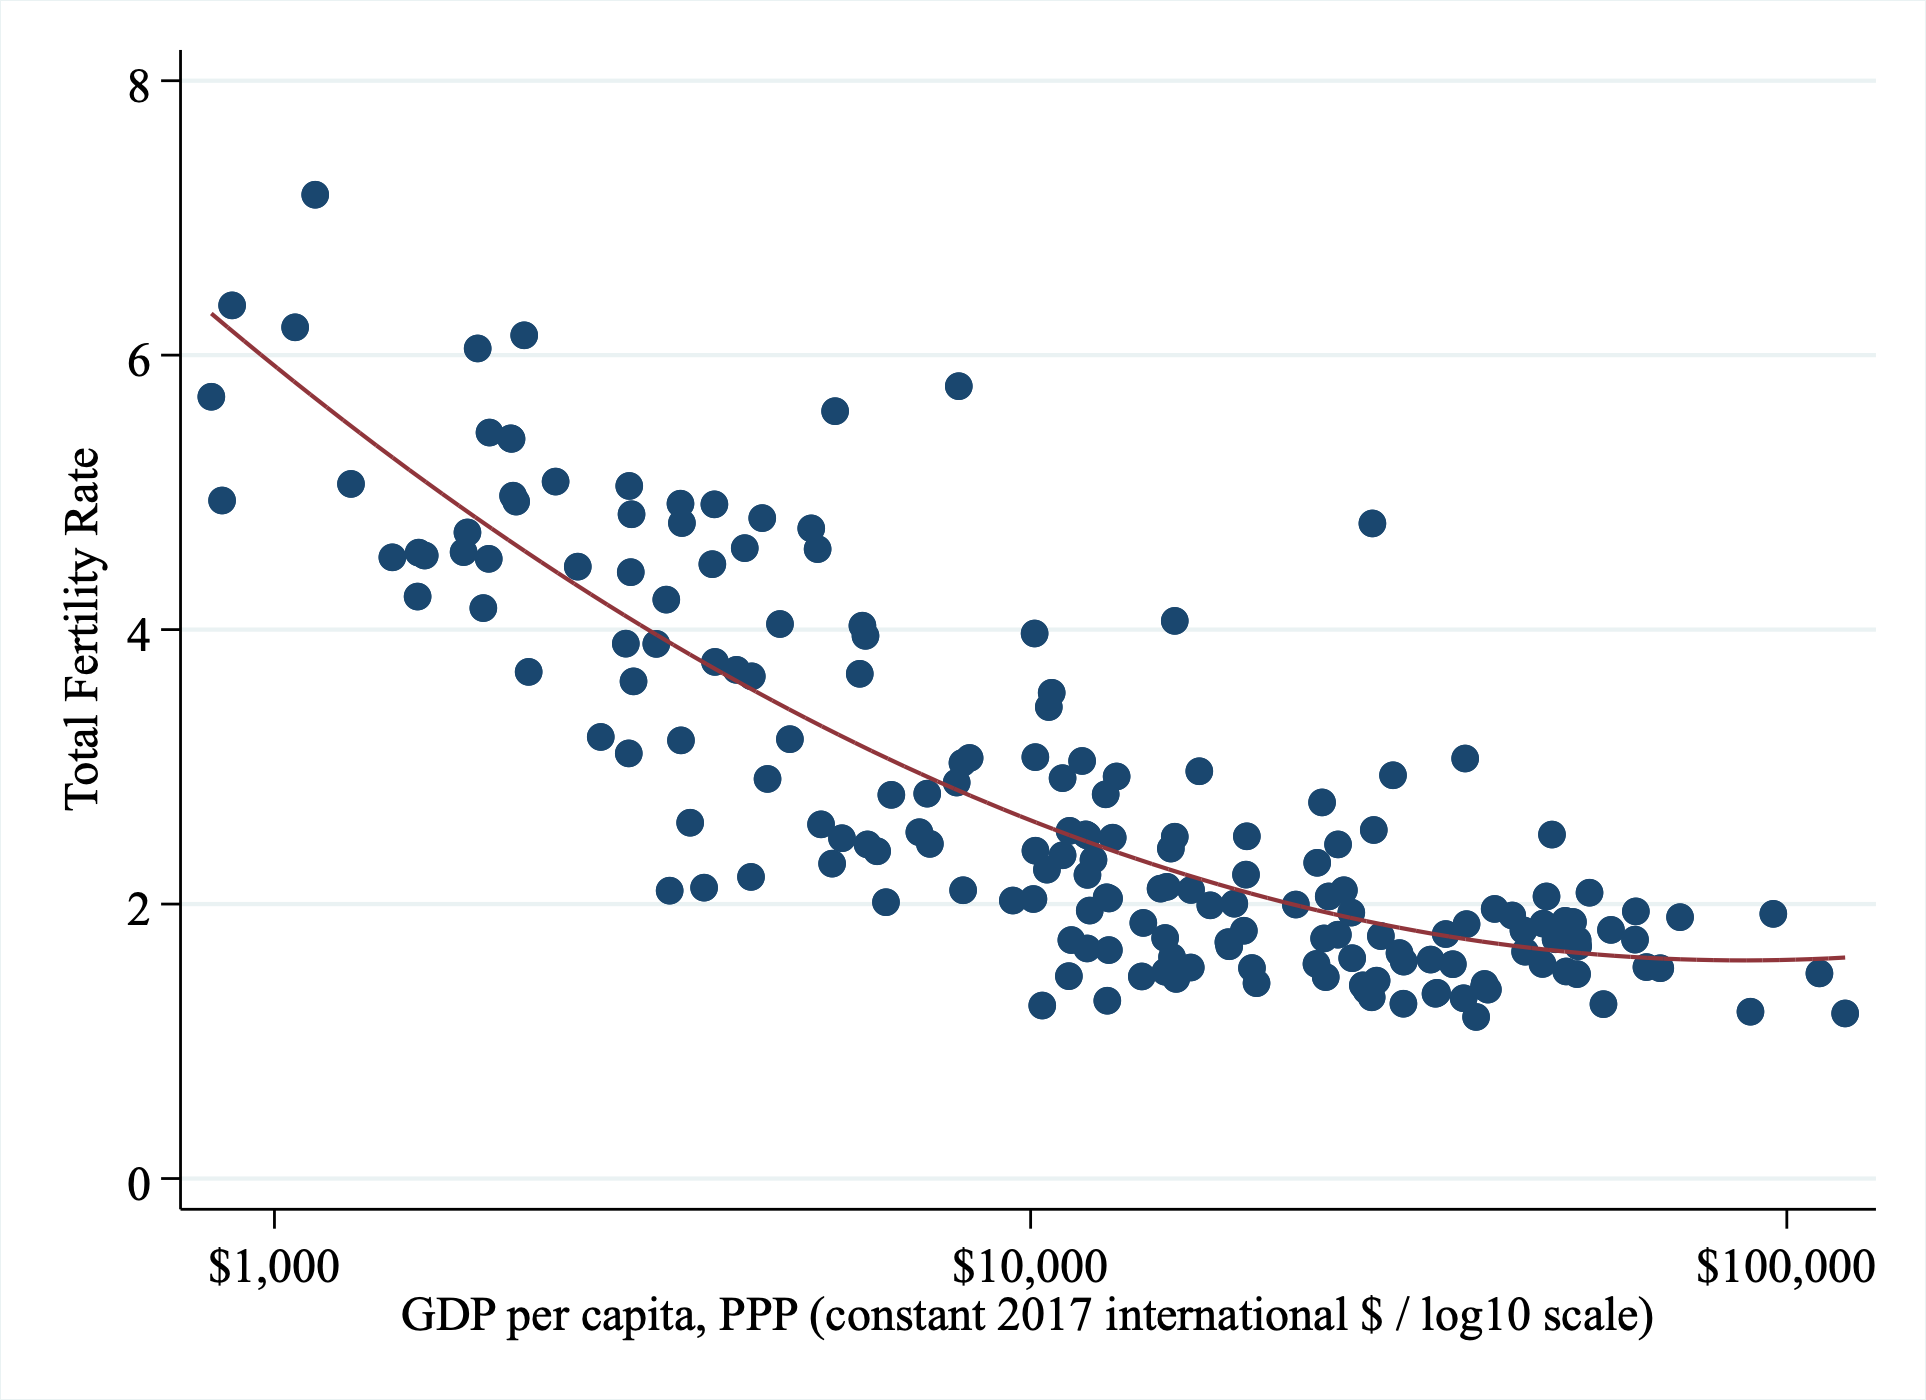
\includegraphics[width=0.8\linewidth]{figures/FC1.jpg}\\
% 	\fontsize{10}{10pt}\selectfont
% 	\flushleft
% 	\emph{Notes:} Each symbol stands for one country. The total fertility rate is defined as the number of children per 1,000 women. The data year is 2020. Data source: Our World in Data \citep{owidfertilityrate,owidgdp}.
% \end{figure}



% \newpage
% \begin{figure}[H]
% 	\centering
% 	\caption{The Relationship Between GDP Per Capita and the Total Fertility Rate}\label{fig.gdp_fertility}
% 	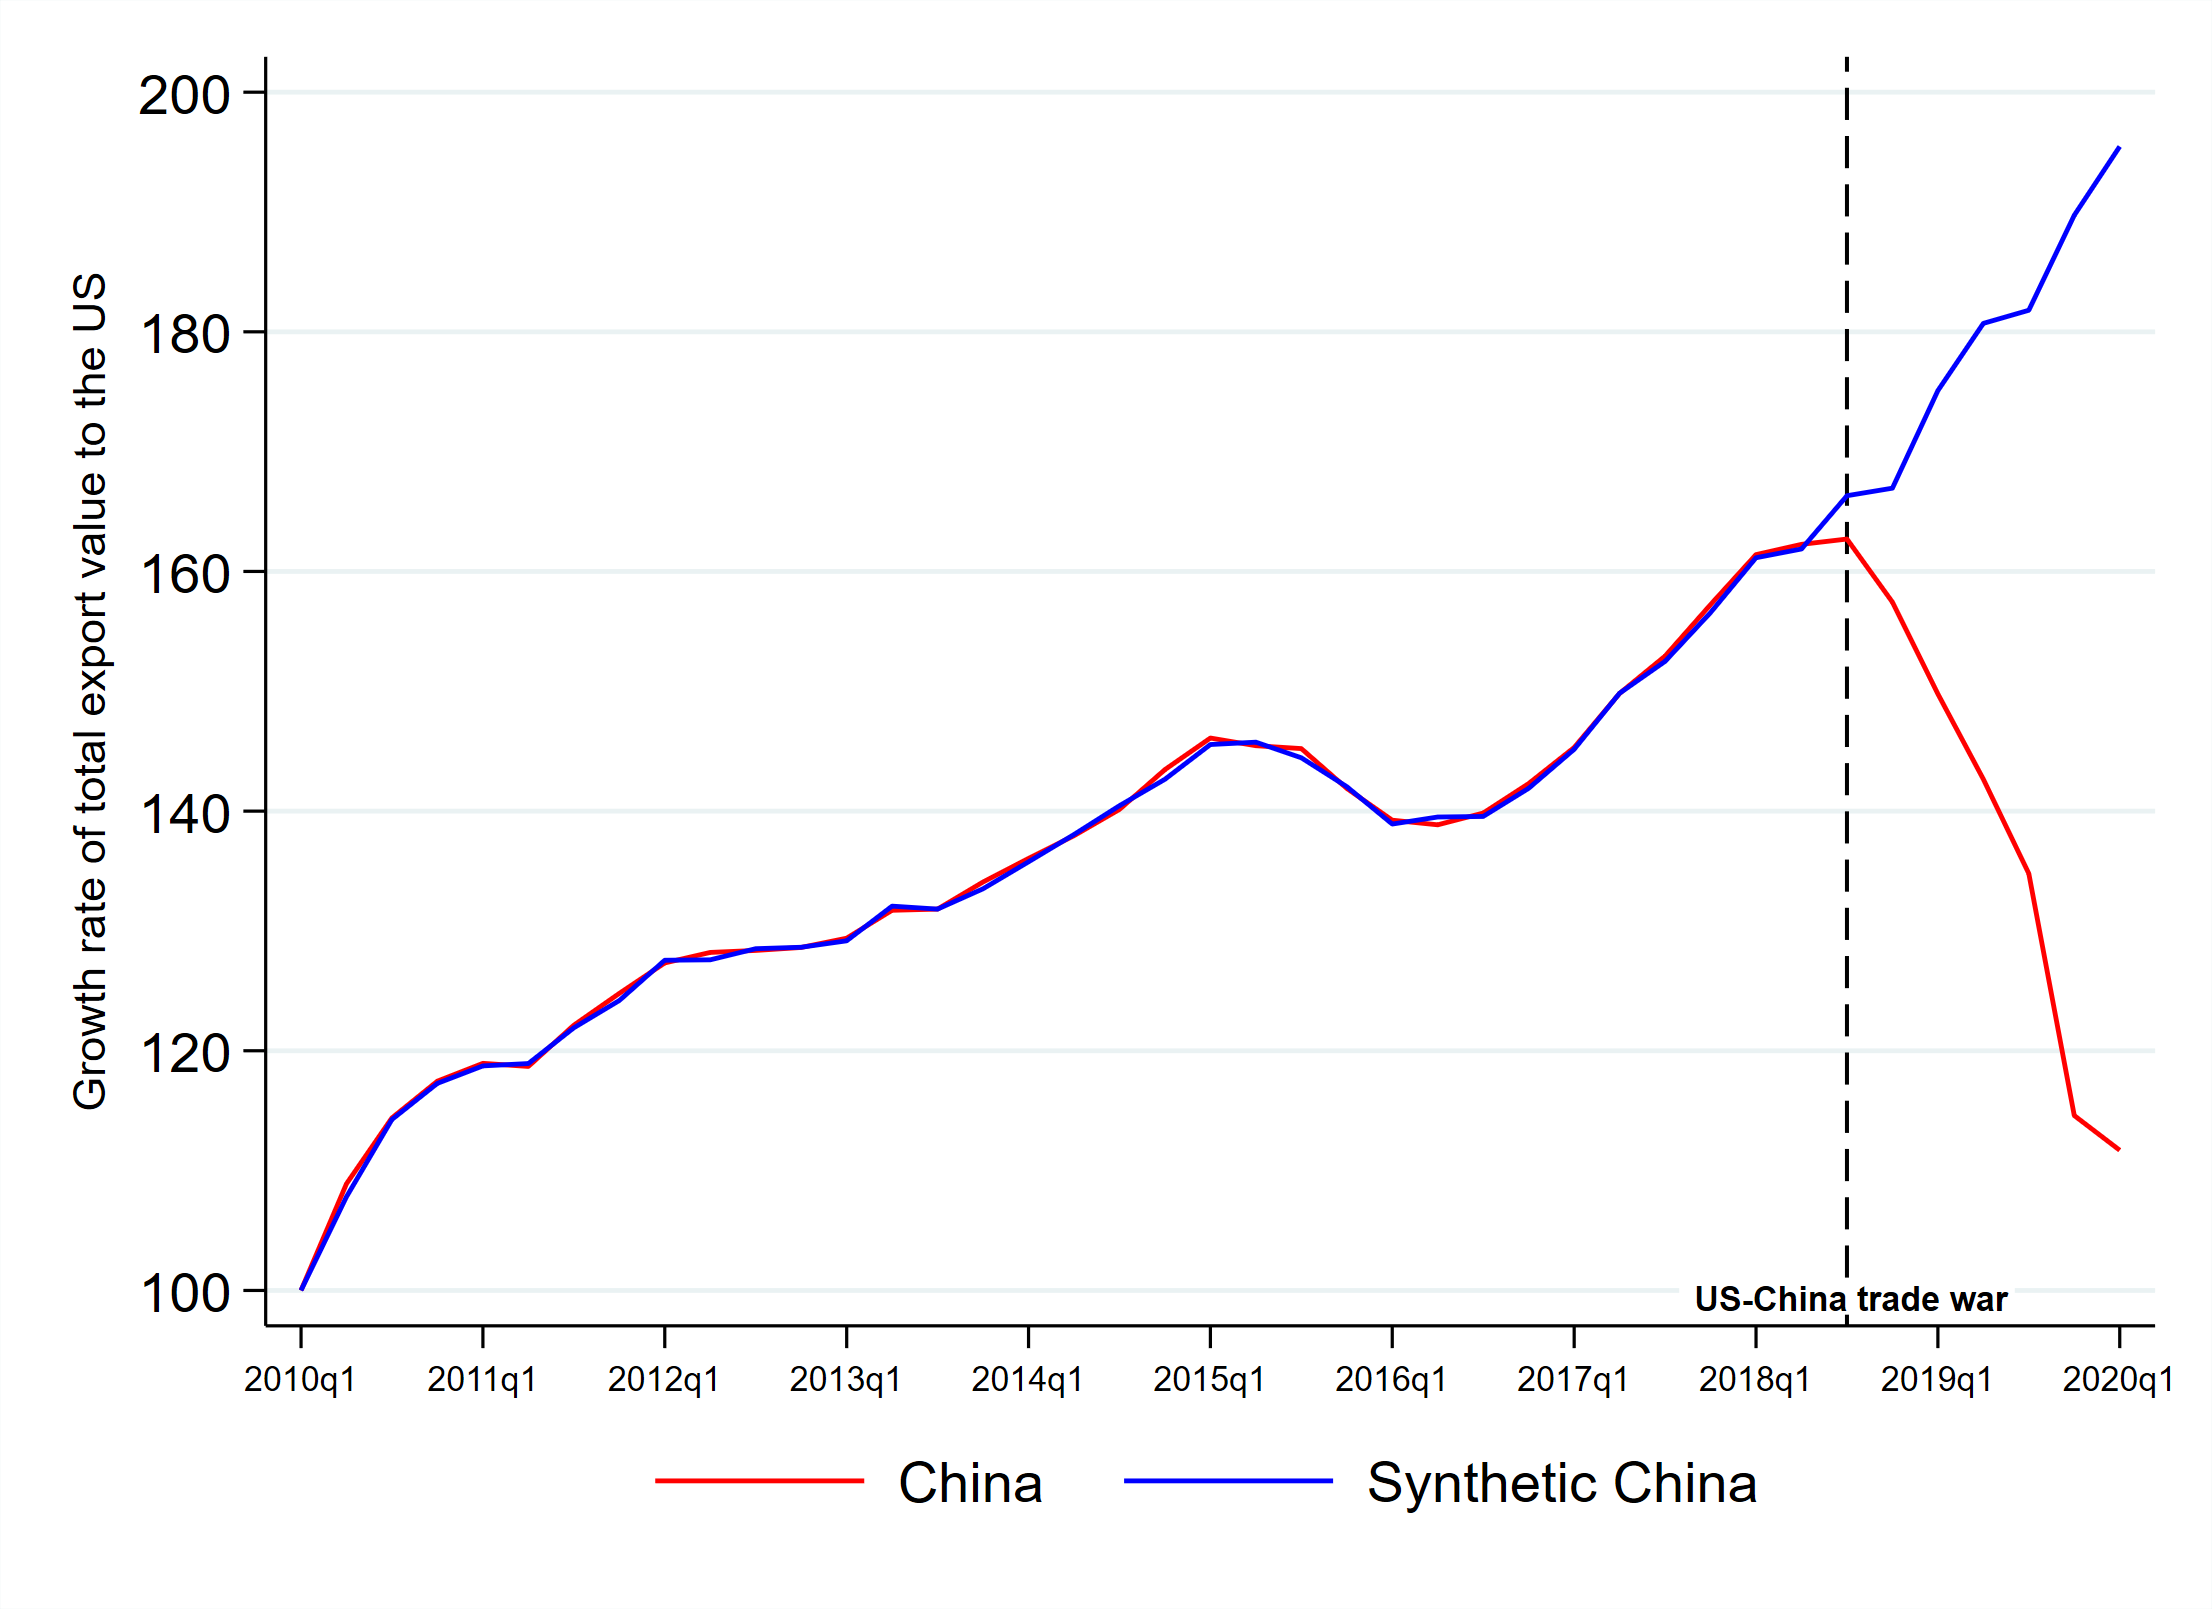
\includegraphics[width=0.8\linewidth]{figures/SCM_us_ch.png}\\
% 	\fontsize{10}{10pt}\selectfont
% 	\flushleft
% 	\emph{Notes:} Each symbol stands for one country. The total fertility rate is defined as the number of children per 1,000 women. The data year is 2020. Data source: Our World in Data \citep{owidfertilityrate,owidgdp}.
% \end{figure}
